%%%%%%%%%%%%%%%%%%%%%%%%%%%%%%%%%%%%%%%%%%%%%%%%%%%%%%%%%%%%%%%%%%%%%%%%%%%%%%%
%Objetivo: Mapeamento Sistemático da Literatura com o objetivo de avaliar o que
%está sendo proposto de melhorias nas funcionalidades das FGRM
%Autor: Vagner Clementino e Rodolfo Resende
%Criação: Ter Out 11 19:03:45 BRT 2016
%Modificação: qua jul 19 22:07:06 -03 2017
%Revisão: ter abr  4 21:13:00 -03 2017
%%%%%%%%%%%%%%%%%%%%%%%%%%%%%%%%%%%%%%%%%%%%%%%%%%%%%%%%%%%%%%%%%%%%%%%%%%%%%%%

\chapter{Mapeamento Sistemático da Literatura}
\label{ch:mapeamento-sistematico}

\section{Introdução}
\label{sec:map-intro}

Neste capítulo apresentamos um Mapeamento Sistemático com o objetivo de
identificar estudos que propõem melhorias das funcionalidades fornecidas pelas
FGRMs. Realizamos a divisão de um conjunto de \textit{64} artigos em dois grupos
pela pertinência do estudo com as seguintes categorias: \textit{(i)}
\textit{dimensões de melhoria}, conforme proposto por Zimmermann e
outros~\cite{zimmermann2009improving} e \textit{(ii)} \textit{função
    desempenhada} no processo de manutenção de software, a partir de um conjunto
de papéis desempenhados por pessoas envolvidas com Manutenção e discutidos por
Polo e outros~\cite{Polo1999}.

A principal contribuição deste mapeamento é uma visão do estado da arte sobre
propostas de melhorias das funcionalidades das FGRMs, com foco especial na
gerenciamento das RMs. Nossa expectativa é que pesquisadores possam encontrar
questões para pesquisa e que profissionais com interesses em FGRMs possam
encontrar discussões e referências neste domínio. Além disso, os desenvolvedores
de FGRMs podem incorporar alguns dos aspectos deste estudo nas funcionalidades
oferecidas pelas FGRMs que são responsáveis.

Este capítulo está organizado conforme descrito a seguir. Na
Seção~\ref{sec:map-metodologia} descrevemos a metodologia adotada através das
perguntas direcionadoras, dos critérios para seleção dos estudos e dos esquemas
de classificação utilizados. Na Seção~\ref{sec:mapeamento_resultados}
apresentamos o resultado do processo de classificar os artigos que fizeram parte
do mapeamento. Uma discussão dos resultados é feita na Seção~\ref{sec:discussao}
As ameaças à validade e os trabalhos relacionados são discutidos nas
Seções~\ref{sec:map_limitacoes_ameacas} e~\ref{sec:map_trabalhos_relacionados},
respectivamente. Um resumo do capítulo é feito na
Seção~\ref{sec:resumo_capitulo}.

\section{Metodologia de Pesquisa}
\label{sec:map-metodologia}

Um \textit{Mapeamento Sistemático da Literatura}, também conhecido como Estudo
de Escopo (Scoping Studies), tem como objetivo fornecer uma visão geral de
determinada área de pesquisa, estabelecer a existência de evidências de estudos
sobre um tema de interesse e fornecer uma indicação da quantidade de trabalhos
na linha de pesquisa sob
análise~\cite{keele2007guidelines,wohlin2012experimentation}. Nesta dissertação
empregamos as diretrizes propostas por Petersen e outros~\cite{Petersen2008} em
que um conjunto de questões de pesquisa é utilizado para guiar a busca e seleção
dos estudos primários. Em seguida, foram construídos esquemas de classificação
com base nos dados extraídos dos artigos. Por fim, foi realizada uma análise
para posicionar os trabalhos em seus respectivos esquemas. A estrutura desta
seção está de acordo com o processo descrito por \textit{Petersen e outros}, de
modo que cada subseção representa uma das etapas propostas pelos autores.

\subsection{Questões de Pesquisa}
\label{subsec:map-questoes-de-pesquisa}

O objetivo deste mapeamento sistemático é identificar novas funcionalidades e
melhorias das existentes que estão sendo propostas na literatura para as FGRMs.
Deste modo, foram definidas as seguintes questões de pesquisa:

\begin{itemize}
	\item \textbf{Questão 01}: \textit{Quais as melhorias e novas
			funcionalidades estão sendo propostas para as FGRM?}
    \item \textbf{Questão 02}: \textit{Para quais papéis envolvidos no processo
            de manutenção de software as melhorias das funcionalidades visam
            dar suporte?}
\end{itemize}

Na \textit{Questão de Pesquisa 01} estamos interessados em entender como a
literatura da área vem propondo melhorias ou apresentando novos comportamentos
para as FGRMs. Estas melhorias devem potencialmente estar relacionadas com os
problemas do gerenciamento das RMs, conforme discutido na
Seção~\ref{ssub:problemas_relacionadas_rm}. O intuito é entender as técnicas e
abordagens adotadas nas soluções propostas. Na \textit{Questão de Pesquisa 02} o
objetivo é descobrir como os diferentes tipos de papéis que fazem parte do
processo de manutenção de software estão recebendo suporte pelos estudos da
área.

\subsection{Pesquisa da Literatura}
\label{subsec:map-pesquisa-literatura}

Para encontrar o conjunto de estudos mais relevantes, bem como eliminar aqueles
que não permitissem responder as questões de pesquisas, adotamos os seguintes
critérios para inclusão ou exclusão de artigos no mapeamento:

\begin{itemize}
	\item Critérios de Inclusão
		\begin{itemize}
			\item Artigos
				publicados em conferências e periódicos (journals)
			\item Estudos
				publicados a partir de 2010\footnote{Foram considerados neste
					estudo artigos publicados até maio/2016, data de realização
					da pesquisa nas base de dados.}
			\item Artigos escritos em
				língua inglesa
			\item Artigos disponíveis com texto
				completo
		\end{itemize}
	\item Critérios de Exclusão
		\begin{itemize}
            \item Livros e literatura cinza (\textit{grey
                  literature}~\cite{keele2007guidelines}), por exemplo,
                  relatórios técnicos, \textit{white papers}, trabalhos em
                  progresso e etc.)
             \item Artigos que não possuem relação com FGRM
			\item Estudos duplicados, neste caso foi considerada a versão mais
				completa do trabalho
		\end{itemize}
\end{itemize}

Os estudos primários foram coletados mediante a aplicação de sentenças de
buscas nas seguintes bases de pesquisa: \textit{IEEE Explore, ACM Digital
    Library, Scopus, e Inspec/Compendex}. No estudo descrito por Dyba e
outros~\cite{dybaa2007applying} verifica-se que o uso de apenas algumas
bibliotecas apresenta um resultado semelhante que uma configuração quase
exaustiva de base de dados. Neste sentido, tomando como base aquele estudo, o
conjunto de bibliotecas digitais utilizada neste mapeamento pode propiciar o
acesso a uma quantidade satisfatória de estudos relevantes. As sentenças de
buscas foram produzidas com base na metodologia PICO (\textit{Population,
    Intervention, Comparison and Outcomes})~\cite{keele2007guidelines} para
ajudar pesquisadores na formulação de termos de busca tomando como ponto de
partida as questões de pesquisa. As sentenças de busca aplicadas em cada base
de pesquisa estão disponíveis no
Apêndice~\ref{ch:app-setenca-de-busca-base-dados}.

Após uma busca automatizada chegamos a um total de 286 artigos\footnote{A lista
    inicial de artigos, após a remoção do duplicados, pode ser acessada
    em~\url{https://archive.org/download/dissertacao-vagner-clementino-um-estudo/artigo-todos-sem-duplicados.csv}}.
A Tabela~\ref{tab:estudos-por-base-dados} exibe o total de estudos recuperados
por base de pequisa. Os trabalhos coletados foram avaliados, através da
ferramenta \textit{JabRef}\footnote{\url{https://www.jabref.org/}}, em busca de
possíveis duplicados. Esta etapa resultou na exclusão de 81 artigos, desta
maneira chegamos a 205 estudos ao final desta etapa do processo.  Finalmente os
trabalhos foram analisados com base na leitura do título e resumo.  Nos casos
em que o título e resumo não eram capazes de indicar que o artigo atendia aos
critérios de inclusão foi realizada uma leitura completa do texto. O processo
descrito resultou em \textbf{64} estudos. A
Figura~\ref{fig:diagrama-processo-selecao} resume a seleção dos estudos
primários através da exibição do número de artigos em cada etapa.

\begin{figure} \centering 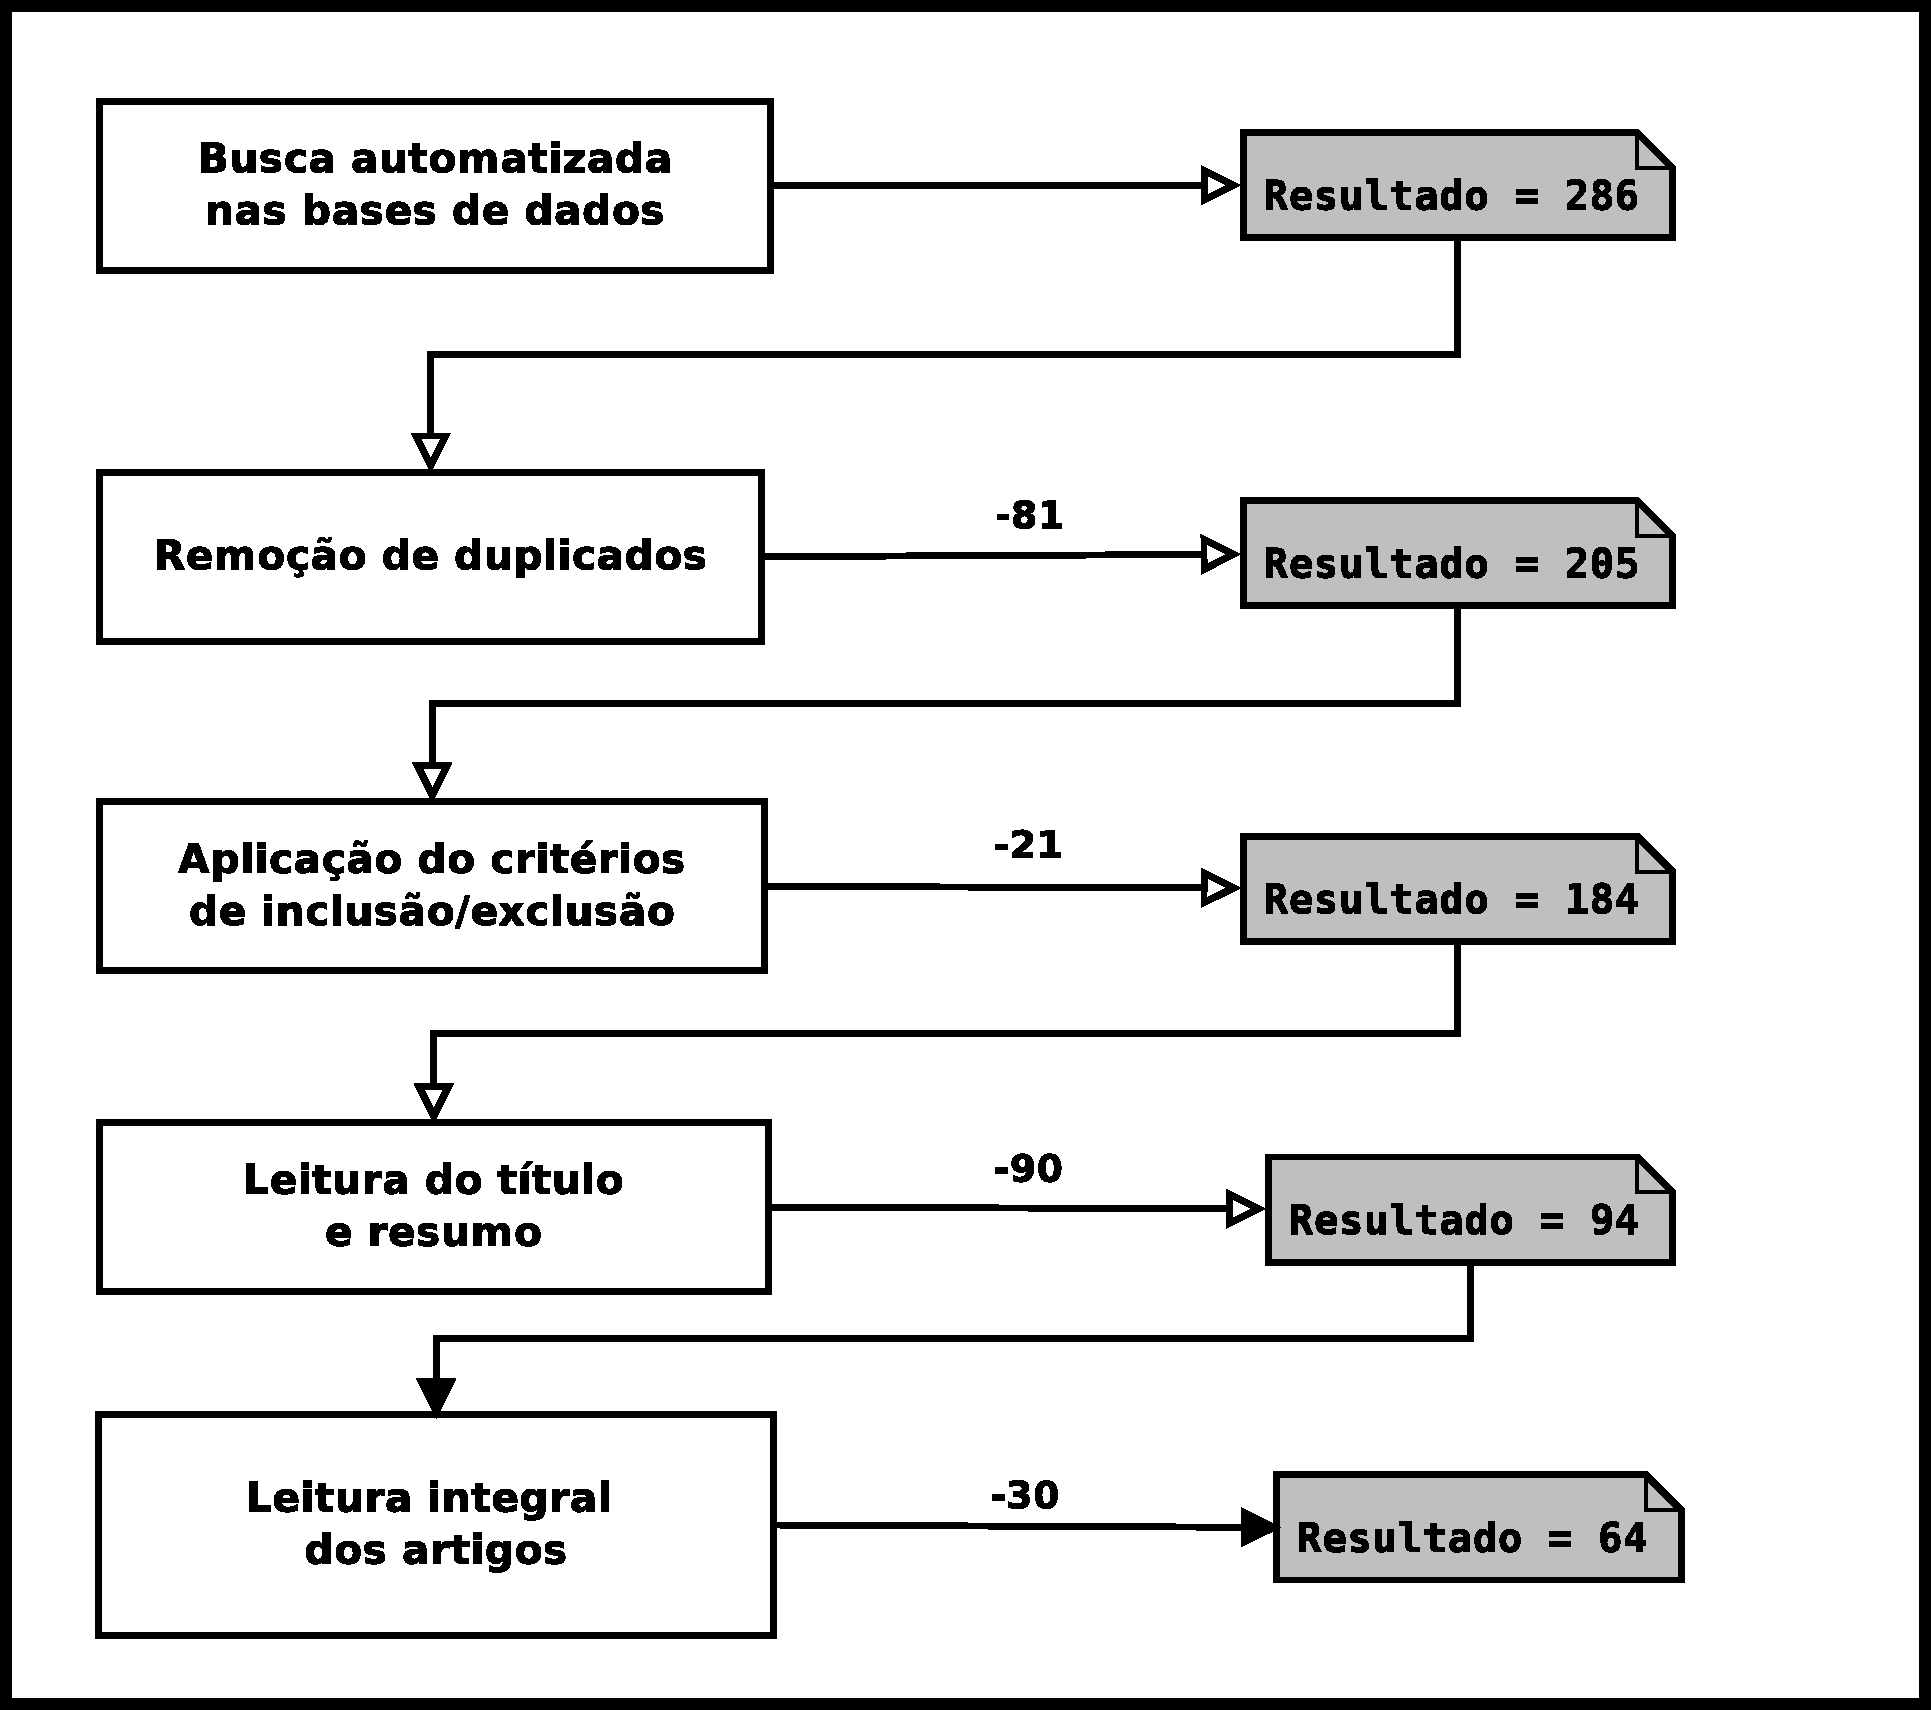
\includegraphics[width=0.75\linewidth]
	{./chapter-mapeamento-sistematico/img/diagrama-processo-selecao.pdf}
	\caption{Número de artigos incluídos durante o processo de seleção dos
		estudos. Figura baseada em~\cite{Petersen2015}}
\label{fig:diagrama-processo-selecao}
\end{figure}

\begin{table}[htb]
	\centering
	\begin{tabular}{cc}
		\toprule
		\textbf{Base de Dados} & \textbf{Total} \\
		\midrule
	   	ACM Digital Library & 109\\
	   	IEEE Explore        & 100\\
		Inspec/Compendex    & 22 \\ 
		Scopus              & 55 \\
		\bottomrule
	\end{tabular}
	\caption{Número de Estudos Recuperados por Base de Dados}
\label{tab:estudos-por-base-dados}
\end{table}

\subsection{Esquemas de Classificação}
\label{subsec:map-esquemas-classificacao}

O mapeamento foi conduzido utilizando dois esquemas de classificação. O primeiro
organiza os artigos pela pertinência com a dimensão de melhoria da
funcionalidade proposta. As dimensões de melhorias foram baseadas no trabalho de
Zimmermann e outros cujo objetivo é aperfeiçoar as funcionalidades das FGRMs de
maneira integral~\cite{zimmermann2009improving}. A segunda classificação
distribui os estudos pelo relacionamento com o suporte dado a determinado papel
no processo de manutenção de software. Entendemos que estes dois esquemas nos
fornecem uma visão de como as melhorias das funcionalidades vêm sendo propostas
tanto do ponto de vista de quem desenvolve quanto das diferentes partes
interessadas dos projetos de software. As pró\-xi\-mas subseções discutem com
mais detalhe cada esquema.

\subsubsection{Classificação por Dimensão de Melhoria}
\label{subsubsec:map-esquema-suporte-problema}

Em um estudo sobre o aperfeiçoamento das FGRMs~\cite{zimmermann2009improving},
os autores argumentam que ter informações completas nos relatos de falhas
(Requisição de Mudança), tão logo quanto possível, ajuda os desenvolvedores a
resolver com mais rapidez o problema. Neste mesmo estudo, eles discutem como
melhorar as funcionalidades oferecidas pelas FGRMs de forma integral, ou seja,
que atenda aos diversos contextos em que este tipo software está integrado.

\begin{description}
	\item[Foco na Informação] Estas melhorias focam diretamente na informação
		fornecida pelo reportador da RM\@. Com ajuda da FGRM, o responsável por
		descrever uma falha, por exemplo, poderia ser motivado a coletar mais
		informações sobre o problema. O sistema poderia verificar a validade e
		consistência do que foi repassado pelo Reportador (detalhes sobre este
		papel pode ser encontrado na
		Subseção~\ref{subsec:man_visao_geral_papeis_na_manutencao_de_software}).
	\item[Foco no Processo] Melhorias com foco no processo visam dar suporte às
		atividades de administração focadas na solução das RMs. Por exemplo, a
        atribuição de RM, poderia ser automatizada visando acelerar o processo.
        Um outro exemplo de melhoria poderia ocorrer no aumento do entendimento
        do progresso realizado em cada RM ou mesmo fornecer ao usuário afetado
        por uma falha a estimativa do tempo necessário para atendimento
        (estimativa de esforço).
	\item[Foco no Usuário] Nesta dimensão estão incluídos tanto os usuários que
		relatam as RMs (Reportadores) quanto os desenvolvedores responsáveis por
        solucioná-las. Os reportadores podem ser orientados sobre qual
        informação fornecer e como coletá-la. Os desenvolvedores também podem se
        beneficiar de um treinamento sobre qual informação esperar e como esta
        informação pode ser utilizada para solucionar determinada RM\@.
	\item[Foco na Ferramenta] As melhorias centradas na ferramenta são
		discutidas com vistas às funcionalidades das FGRMs\@. Elas podem reduzir
		a complexidade da coleta e fornecimento das informações necessárias para
		solucionar a RM\@. Por exemplo, as FGRMs poderiam ser configuradas para
		automaticamente identificar a cadeia de registros de ativação de funções
        (\textit{stack trace}) e adicioná-la ao erro reportado. A ferramenta
        poderia ainda simplificar o processo de reprodução do erro mediante a
        captura automatizada de tela (\textit{screenshots}).
\end{description}

Para a classificação dos estudos nos esquemas utilizados foi realizado um
processo baseado no trabalho de Petersen e outros~\cite{Petersen2008}, que é
composto por duas etapas:

\begin{enumerate}[I]
	\item análise das palavras-chaves e conceitos que
		identificam as contribuições do estudo por meio da analise do título e
		resumo.
	\item combinações das palavras-chaves para construir um conjunto de
		categorias para classificação dos artigos.
\end{enumerate}

Os autores recomendam que nos casos em que o resumo e o título do estudo não
sejam capazes de caracterizá-lo, as seções de introdução e conclusão também
devem ser analisadas. Para as bases de pesquisa de dados em que era informado
mais de um conjunto de palavras-chaves para um mesmo artigo, utilizamos aquelas
que foram definidas pelos autores. Mediante a aplicação do processo descrito foi
construído o esquema de classificação apresentado na
Figura~\ref{fig:diagrama-esquema-dimensao-melhorias}.

\begin{figure}[tb] \centering
	\makebox[\textwidth]{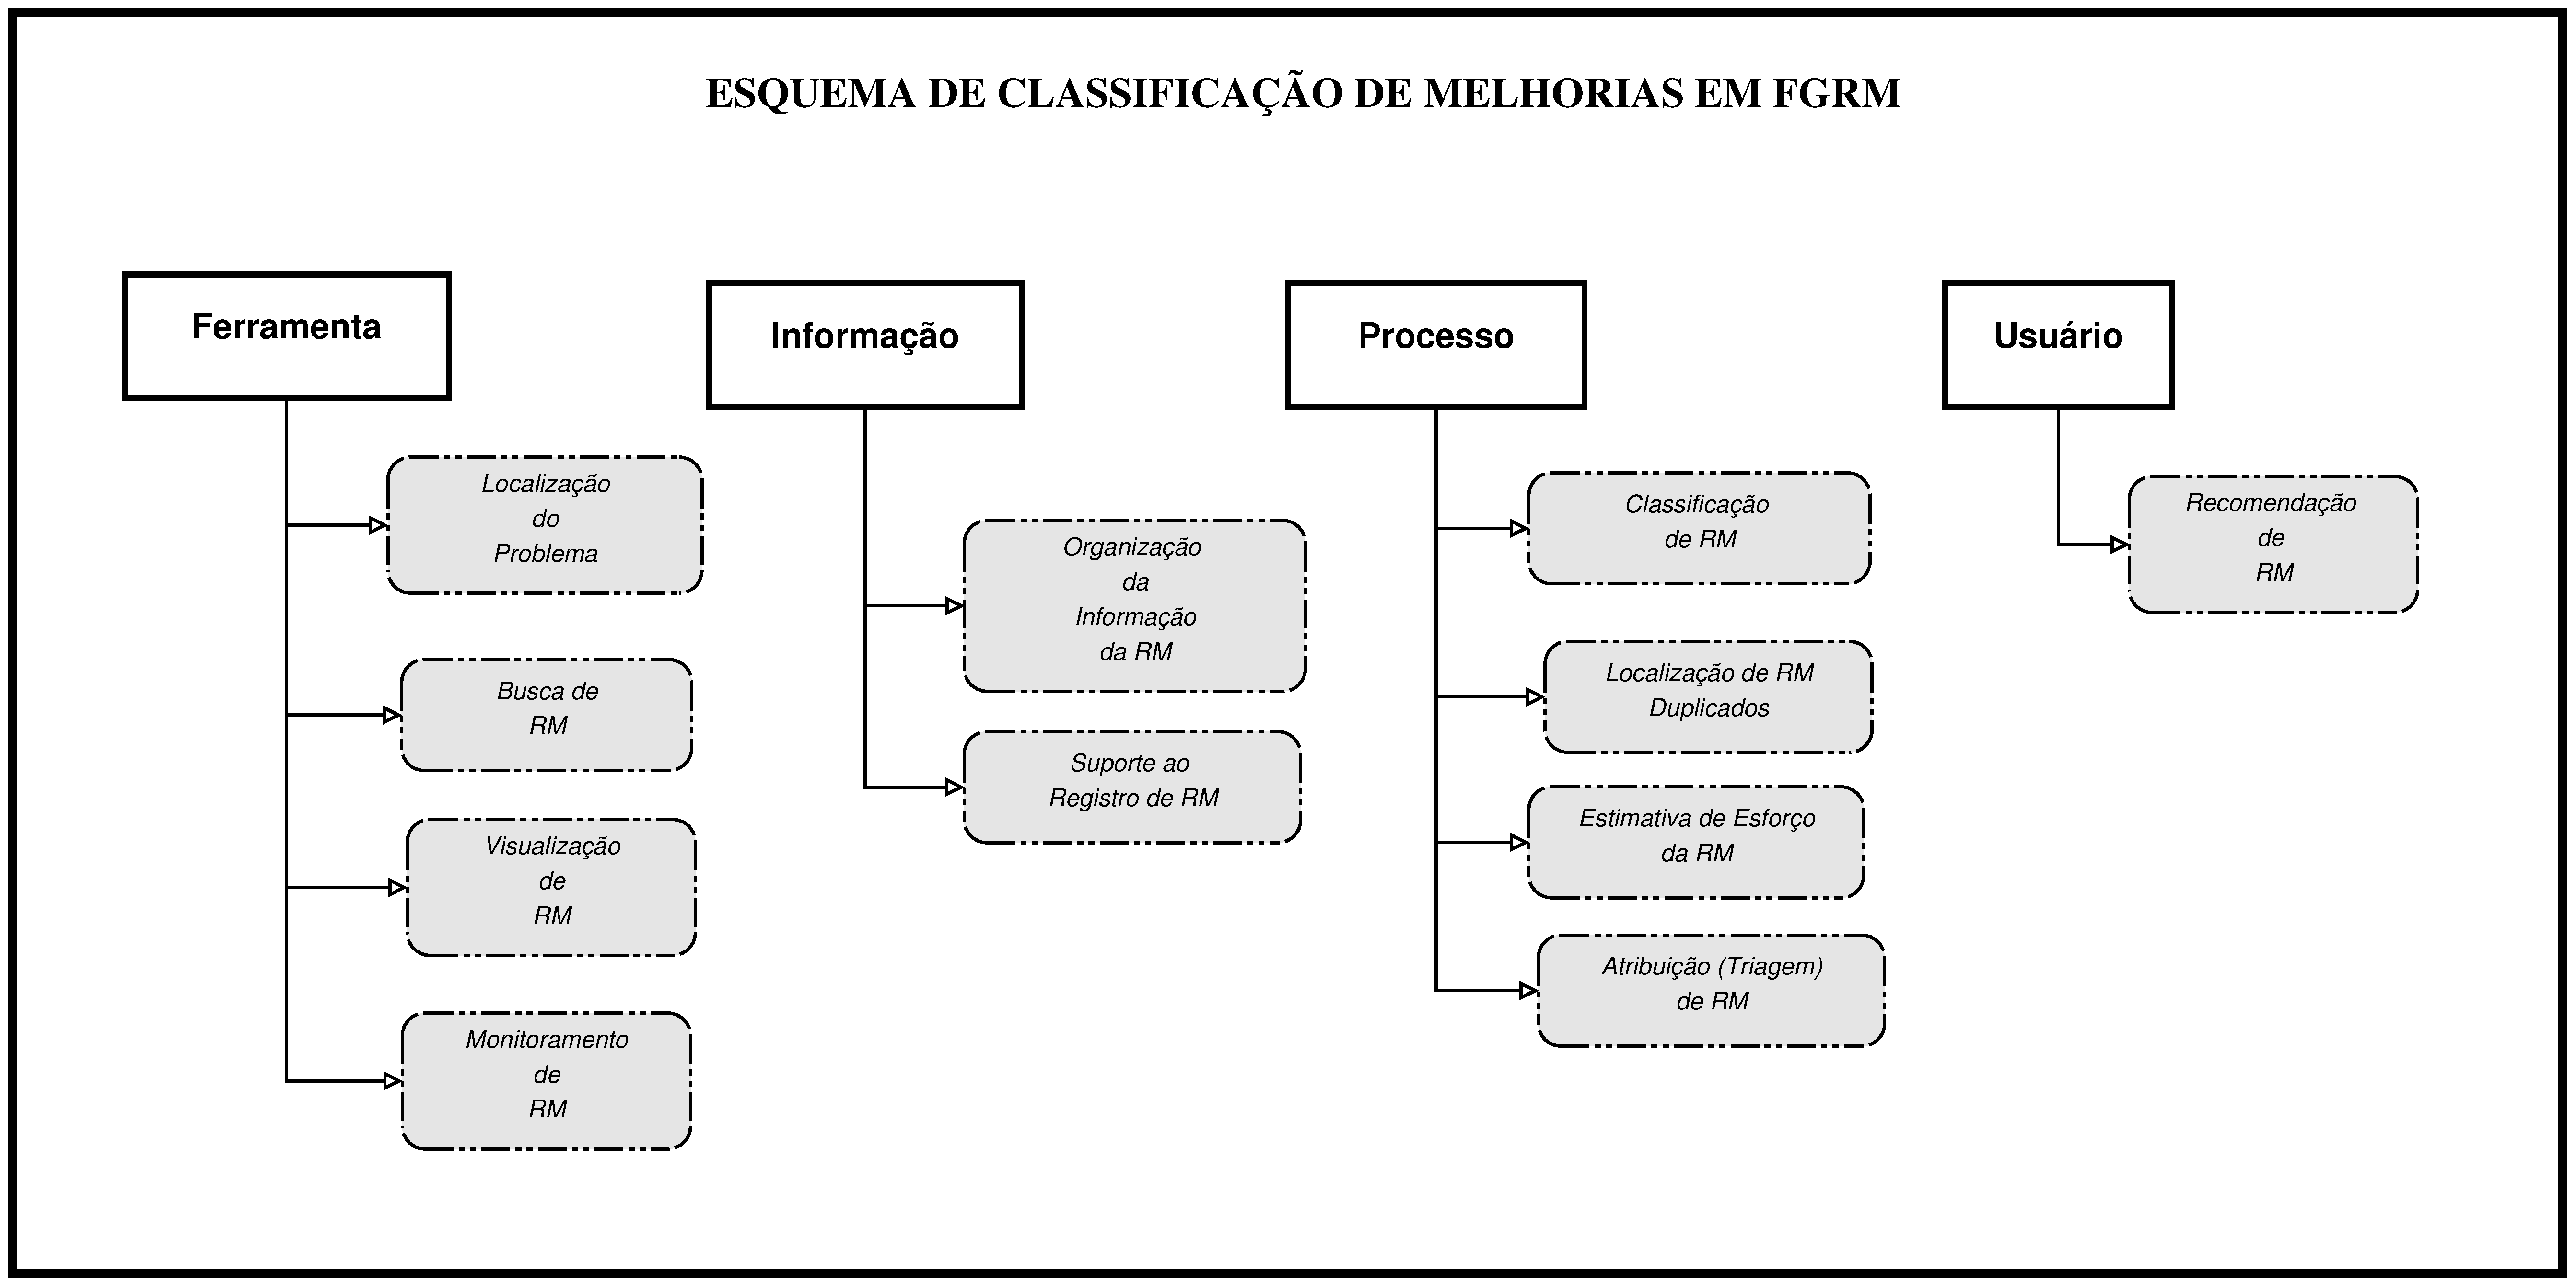
\includegraphics[width=.7\paperwidth]{./chapter-mapeamento-sistematico/img/diagrama-esquema-dimensoes-melhorias.eps}}
    \caption{Esquema de classificação das melhorias propostas na literatura. Os
        retângulos representam as dimensões de melhorias e os polígonos de
        cantos arredondados representam tópicos de problemas do gerenciamento
        das RMs.}
\label{fig:diagrama-esquema-dimensao-melhorias}
\end{figure}

\subsubsection{Classificação por Suporte ao Papel da Manutenção de Software}
\label{subsubsec:map-esquema-suporte-papel-man}

Neste esquema de classificação estamos interessado em avaliar como os estudos
dão suporte aos papéis apresentados na
Subseção~\ref{subsec:man_visao_geral_papeis_na_manutencao_de_software}. A
construção da classificação utiliza a mesma metodologia descrita na seção
anterior e utilizada a classificação de papéis da manutenção proposto por Polo e
outros~\cite{Polo1999}.

\section{Resultados}
\label{sec:mapeamento_resultados}

Nesta seção apresentamos os estudos divididos para cada um dos esquemas de
classificação utilizados. Iniciamos com uma análise da frequência de publicação
sobre o tema do mapeamento e posteriormente apresentamos os resultados para cada
uma das dimensões de melhoria. Seguimos com a análise dos estudos pelo papel ao
qual a funcionalidade proposta visa dar suporte.

A frequência de publicação dos estudos teve em 2010, primeiro ano do período
analisado, um total de 05 trabalhos publicados. A maior quantidade de
publicação ocorreu entre os anos de 2012, 2013 e 2014, com, respectivamente,
14, 12 e 13 artigos. No ano de 2016, último ano do período de referência,
encontramos 03 estudos publicados. A Tabela~\ref{tab:publicacao_por_ano} exibe
o número de estudos primários identificados entre os anos de 2010 e 2016,
período de referência utilizado no mapeamento.

\begin{table}[htpb]
\centering
\resizebox{.25\textwidth}{!}{%
\begin{tabular}{@{}lc@{}}
\toprule
\textbf{Ano} & \textbf{Frequência} \\ \midrule
2010         & 5                   \\
2011         & 8                   \\
2012         & 14                  \\
2013         & 12                  \\
2014         & 13                  \\
2015         & 9                   \\
2016         & 3                   \\ \bottomrule
\end{tabular}%
}
\caption{Número de estudos primários por ano de publicação.}
\label{tab:publicacao_por_ano}
\end{table}

\subsection{Classificação por Dimensões de Melhoria}
\label{sub:extensões_para_problemas_na_manutenção_de_software}

Nesta seção apresentamos estudos relacionados com a dimensão denominada
``Melhoria das funcionalidades das FGRMs\@''. A classificação está estruturada
de modo que no primeiro nível temos uma das quatro dimensões de melhorias
discutidas na Subseção~\ref{subsubsec:map-esquema-suporte-problema}. O segundo
nível é composto por tópicos que são os problemas do gerenciamento das RMs. Uma
discussão mais detalhada sobre estes problemas pode ser encontrada na
Subseção~\ref{ssub:problemas_relacionadas_rm}. A
Tabela~\ref{tab:taxonomia-problemas-manutencao} exibe a distribuição dos
estudos pela dimensão de melhoria e o seu respectivo tópico.

% Inclusão da tabela
\begin{table}[htbp]
\centering
\caption{My caption}
\label{my-label}
\resizebox{\textwidth}{!}{%
\begin{tabular}{|c|l|l|c|}
\hline
\textbf{Dimensão da Melhoria} & \multicolumn{1}{c|}{\textbf{Tópico}}             & \multicolumn{1}{c|}{\textbf{Estudos}}          & \textbf{Total}       \\ \hline
\multirow{13}{*}{Ferramenta}  & Busca de RM                                      & \cite{Liu2014}                                 & 1                    \\ \cline{2-4} 
                              & \multirow{7}{*}{Localização do Problema}         & \cite{Bangcharoensap:2012:LSC:2419061.2419428} & \multirow{7}{*}{7}   \\
                              &                                                  & \cite{Corley2011}                              &                      \\
                              &                                                  & \cite{Nguyen:2012:MAR:2393596.2393671}         &                      \\
                              &                                                  & \cite{Romo:2015:TAT:2745802.2745833}           &                      \\
                              &                                                  & \cite{thung2013automatic}                      &                      \\
                              &                                                  & \cite{Thung:2014:BIT:2635868.2661678}          &                      \\
                              &                                                  & \cite{Wong:2014:BBF:2705615.2706096}           &                      \\ \cline{2-4} 
                              & Monitoramento de RM                              & \cite{Aggarwal:2014:MIT:2593801.2593810}       & 1                    \\ \cline{2-4} 
                              & \multirow{4}{*}{Visualização de RM}              & \cite{dal2013closer}                           & \multirow{4}{*}{4}   \\
                              &                                                  & \cite{Hora2012}                                &                      \\
                              &                                                  & \cite{Sasso2014}                               &                      \\
                              &                                                  & \cite{takama2013application}                   &                      \\ \hline
\multirow{9}{*}{Informação}   & \multirow{2}{*}{Organização da Informação da RM} & \cite{mani2012ausum}                           & \multirow{2}{*}{2}   \\
                              &                                                  & \cite{Otoom2016}                               &                      \\ \cline{2-4} 
                              & \multirow{7}{*}{Suporte ao Registro da RM}       & \cite{Bettenburg2008a}                         & \multirow{7}{*}{7}   \\
                              &                                                  & \cite{Correa2013b}                             &                      \\
                              &                                                  & \cite{moran2015auto}                           &                      \\
                              &                                                  & \cite{Moran:2015:EAA:2786805.2807557}          &                      \\
                              &                                                  & \cite{Tu:2014:MQI:2677832.2677844}             &                      \\
                              &                                                  & \cite{White:2015:GRR:2820282.2820291}          &                      \\
                              &                                                  & \cite{Wu2011a}                                 &                      \\ \hline
\multirow{40}{*}{Processo}    & \multirow{12}{*}{Atribuição (Triagem) de RM}     & \cite{Banitaan2013}                            & \multirow{12}{*}{12} \\
                              &                                                  & \cite{hosseini2012market}                      &                      \\
                              &                                                  & \cite{Hu:2014:EBT:2707683.2708297}             &                      \\
                              &                                                  & \cite{Naguib2013}                              &                      \\
                              &                                                  & \cite{Nagwani2012}                             &                      \\
                              &                                                  & \cite{shokripour2012automatic}                 &                      \\
                              &                                                  & \cite{tian2015automated}                       &                      \\
                              &                                                  & \cite{ValdiviaGarcia:2014:CPB:2597073.2597099} &                      \\
                              &                                                  & \cite{Wu2011}                                  &                      \\
                              &                                                  & \cite{Xuan:2012:DPB:2337223.2337227}           &                      \\
                              &                                                  & \cite{Zanetti2013}                             &                      \\
                              &                                                  & \cite{Zhang2014}                               &                      \\ \cline{2-4} 
                              & \multirow{10}{*}{Classificação de RM}            & \cite{behl2014bug}                             & \multirow{10}{*}{10} \\
                              &                                                  & \cite{chawla2015automated}                     &                      \\
                              &                                                  & \cite{Gegick2010}                              &                      \\
                              &                                                  & \cite{Izquierdo2015}                           &                      \\
                              &                                                  & \cite{kochhar2014automatic}                    &                      \\
                              &                                                  & \cite{Nagwani2013}                             &                      \\
                              &                                                  & \cite{netto2010automated}                      &                      \\
                              &                                                  & \cite{somasundaram2012automatic}               &                      \\
                              &                                                  & \cite{Tian:2013:DPP:2550526.2550574}           &                      \\
                              &                                                  & \cite{zhang2011bug}                            &                      \\ \cline{2-4} 
                              & \multirow{5}{*}{Estima de Esforço da RM}         & \cite{Bhattacharya:2011:BTP:1985441.1985472}   & \multirow{5}{*}{5}   \\
                              &                                                  & \cite{Nagwani2010}                             &                      \\
                              &                                                  & \cite{Thung2012}                               &                      \\
                              &                                                  & \cite{Vijayakumar2014}                         &                      \\
                              &                                                  & \cite{xia2015automatic}                        &                      \\ \cline{2-4} 
                              & \multirow{13}{*}{Localização de RM Duplicados}   & \cite{alipour2013contextual}                   & \multirow{13}{*}{13} \\
                              &                                                  & \cite{banerjee2012automated}                   &                      \\
                              &                                                  & \cite{hindle2016contextual}                    &                      \\
                              &                                                  & \cite{Koopaei:2015:CAD:2886444.2886474}        &                      \\
                              &                                                  & \cite{Lerch:2013:FDY:2495256.2495763}          &                      \\
                              &                                                  & \cite{Liu:2012:TBR:2393596.2393628}            &                      \\
                              &                                                  & \cite{Prifti2011}                              &                      \\
                              &                                                  & \cite{Song2010a}                               &                      \\
                              &                                                  & \cite{sun2010discriminative}                   &                      \\
                              &                                                  & \cite{Sun2011}                                 &                      \\
                              &                                                  & \cite{Thung2014}                               &                      \\
                              &                                                  & \cite{Tian2012}                                &                      \\
                              &                                                  & \cite{Tomasev2013}                             &                      \\ \hline
\multirow{2}{*}{Usuário}      & \multirow{2}{*}{Recomendação de RM}              & \cite{malheiros2012source}                     & \multirow{2}{*}{2}   \\
                              &                                                  & \cite{Wang2011a}                               &                      \\ \hline
\end{tabular}%
}
\end{table}


\subsubsection{Melhorias Propostas na Dimensão Ferramenta}
\label{ssub:melhorias_dim_ferramenta}

Este ramo do esquema de classificação inclui os estudo que possuem relação com
tópicos como Localização do Problema e Visualização de RMs.

\paragraph{Localização do Problema:}

Os estudos incluídos neste tópico focam em localizar a origem de um problema de
software com base nos dados da RM~\cite{Hovemeyer:2004:FBE:1052883.1052895}.
Com objetivo de melhorar a eficiência da localização de um problema, diversas
informações contidas nas RMs estão sendo utilizadas. As abordagens propostas
utilizam informações como cadeia de registros de
ativação~\cite{Wong:2014:BBF:2705615.2706096}, des\-cri\-ção e campos
estruturados das RMs~\cite{Thung:2014:BIT:2635868.2661678} e os históricos de
versões do código fonte do
sistema~\cite{Bangcharoensap:2012:LSC:2419061.2419428, corley2011recovering,
    Romo:2015:TAT:2745802.2745833}. Algumas das melhorias propostas foram
incluídas em ferramentas largamente empregadas no mercado utilizando os
mecanismos de extensão que elas oferecem. A ferramenta
\textit{BugLocalizer}\footnote{\url{https://github.com/smagsmu/buglocalizer}},
implementada como extensão do Bugzilla, extrai o texto do sumário e do relato
de uma RM e calcula a semelhança entre o texto relatado e o código fonte para
encontrar os arquivos onde a falha possivelmente está
localizada~\cite{Thung:2014:BIT:2635868.2661678}. A ferramenta
\textit{BugTrace}~\cite{corley2011recovering} é uma extensão do Bugzilla que
implementa uma abordagem que analisa os \textit{patches}\footnote{Um
    \textit{patch} é um software projetado para atualizar um programa de
    computador ou seus dados de suporte, para corrigi-lo ou melhorá-lo.}
inseridos em RM para determinar um elo de rastreabilidade entre uma falha e o
código fonte.

\paragraph{Visualização de RM:}

Os estudos neste tópico estão relacionados com melhoria da visualização da
informação contida na RM\@. Com o objetivo de apresentar diferentes formas de
visualizar os dados de uma RM novos conceitos estão sendo propostos. No estudo
de Hora e outros~\cite{hora2012bug} é apresentado o conceito de Mapas de
Defeitos (\textit{BugsMaps)} que mostra a RM e uma ligação dela com outros
artefatos de software, por exemplo, o histórico de versões. O conceito de
hiperligação entre documentos é utilizado para permitir a navegação entre os
artefatos que estão relacionados a uma RM~\cite{dal2014bug}.

Verificamos ainda no artigo proposto por Takama e
Kurosawa~\cite{takama2013application} a aplicação de tecnologias de
visualização de informação empregada para o monitoramento das informações
contidas nas RMs. Uma FGRM atualiza quase toda informação de uma RM como texto,
sem maiores estruturações. A solução proposta pelos autores visa suportar o
monitoramento das RMs apresentando ao usuário da FGRM, seja ele o afetado por
uma falha, o responsável por relatar a requisição ou mesmo um membro da equipe
de manutenção, a situação das RMs mediante animações produzidas com base nas
atualizações ocorridas nas mesmas.

Por conta da natureza das melhorias propostas neste tópico de pesquisa,
verificamos que diversos estudos foram implementados como protótipos. Desta
forma, é possível avaliar as propostas contidas neste tópico através das
ferramentas como o
\textit{bugMaps}\footnote{\url{http://rmod.lille.inria.fr/web/pier/software/BugMaps}}~\cite{hora2012bug}
e \textit{In* Bug}\footnote{\url{http://inbug.inf.usi.ch}}~\cite{dal2014bug}.

\subsubsection{Melhorias Propostas na Dimensão Informação}
\label{ssub:melhorias_dim_informacao}

Apresentamos os trabalhos relacionados à melhoria da qualidade da informação de
uma RM\@. A melhoria pode envolver suporte ao registro de uma RM antes que ela
seja armazenada no Repositório de RMs; a melhoria também pode envolver a
organização da informação contida no relato para facilitar o entendimento pelos
desenvolvedores e demais profissionais envolvidos na manutenção de software.

\paragraph{Suporte ao Registro da RM:}

Para melhorar a qualidade da informação fornecida nas RMs os artigos sobre o
tema, em sua maioria, definem um limiar para algum atributo do texto
correspondente ao relato da RM\@. Caso este limiar não seja alcançado alguma
ação é tomada, como por exemplo, a exibição de uma mensagem de alerta para o
responsável pela criação da RM\@. A determinação do que seria um boa descrição
de um problema de software foi obtida mediante uma pesquisa com profissionais
envolvidos com manutenção de software no estudo de Zimmermann e
outros~\cite{zimmermann2010makes}. Em outro estudo os próprios autores
definiram as métricas que posteriormente foram utilizadas para avaliar o relato
da RM~\cite{Tu:2014:MQI:2677832.2677844}.

Um segundo nicho de estudos visa suportar a reprodução da falha do software.
Estes estudos incluem tanto registrar o conjunto de ações que resultaram na
falha~\cite{White:2015:GRR:2820282.2820291}, quanto em autocompletar o texto que
compõe o relato de uma falha~\cite{moran2015auto}. Um ponto em comum deste dois
estudos é que eles foram pensados para o ambiente de desenvolvimento de
aplicações para dispositivos móveis, mais especificamente para dispositivos
baseados no sistema Android\footnote{\url{https://www.android.com/}}. Uma
possível justificativa para o foco em aplicações móveis pode ser a dificuldade
em registrar uma falha neste tipo de
ambiente~\cite{White:2015:GRR:2820282.2820291, moran2015auto}.

Muitos dos estudos resultaram em ferramentas com a finalidade de realizar uma
prova de conceito sobre como ajudar ao Reportador a fornecer um relato de boa
qualidade~\cite{Tu:2014:MQI:2677832.2677844, zimmermann2010makes,
    Wu2011a,White:2015:GRR:2820282.2820291,moran2015auto}.

\paragraph{Organização da Informação da RM:}

Em diversas situações o desenvolvedor precisa examinar manualmente o relato das
RMs que podem variar em tamanho e complexidade~\cite{mani2012ausum}. Neste
contexto, o resumo (sumarização) automático do texto contido em uma RM é uma
maneira de reduzir a quantidade de dados que o desenvolvedor precisa analisar.
A ferramenta denominada AUSUM~\cite{mani2012ausum} propõe uma abordagem,
utilizando técnicas não supervisionadas de aprendizado de máquina, para aprender
e sumarizar um ou mais relatos relacionados.

\subsubsection{Melhorias Propostas na Dimensão Processo}
\label{ssub:melhorias_dim_processo}

\paragraph{Identificação de RMs Duplicadas}

O processo de identificação de RMs duplicadas consiste em avaliar se
determinado relato já foi realizado em algum outro momento.  A literatura
discute dois tipos de tratamento para o problema~\cite{kaushik2012comparative,
    Tian2012}:

\begin{enumerate}[(i)]

	\item remoção de duplicadas

	\item identificação de duplicatas

\end{enumerate}

No primeiro tipo, o objetivo é evitar que RMs duplicadas entrem no repositórios
de RMs e, desta forma, evitar o esforço e o tempo extra necessário para
identificá-las posteriormente. Por outro lado, no segundo tipo o objetivo é
sugerir uma lista de possíveis duplicatas durante o processo de registro de uma
nova RM\@. Um ponto importante é que o segundo tipo se baseia na premissa que
registrar um mesmo problema por mais de uma vez nem sempre é ruim, já que a
possível ``cópia'' pode fornecer informações
adicionais~\cite{bettenburg2008duplicate}. É importante que novas abordagens
tentem equilibrar estes dois tipos de tratamento para evitar o tempo extra para
análise de uma RM bem como apoiar os desenvolvedores com informações
adicionais~\cite{Lerch:2013:FDY:2495256.2495763,Thung2014}.

Uma forma de tratar o problema é utilizar modelos de espaços vetoriais para
medir a similaridade entre as RMs~\cite{liu2014faceted, sun2010discriminative,
    Thung2014,tomavsev2013exploiting}. Outros trabalhos tentam utilizar técnicas
em que os termos específicos do domínio do projeto de software, contidos no
relato das RMs, são utilizados na determinação da probabilidade que duas
requisições sejam duplicadas~\cite{hindle2016contextual, alipour2013contextual}.
Em resumo verificamos que o relato contido na RM é utilizado como fonte de
informação para técnicas de Re\-cu\-pe\-ra\-ção da Informação visando determinar
a similaridade entre duas RMs.

\paragraph{Atribuição de RM:}

Os estudos apresentados neste tópico foram classificados pela pertinência com a
automatização do processo de encontrar o desenvolvedor mais apto para solucionar
determinada RM\@. A principal fonte de informação utilizada nas abordagens
propostas é o relato contido na RM, todavia, outros dados são utilizados, tais
como a prioridade~\cite{tian2015automated}, registros (log) do sistema de
controle de versão~\cite{shokripour2012automatic, Hu:2014:EBT:2707683.2708297} e
itens do contexto do projeto como por exemplo: o perfil e preferências do
desenvolvedor, quantidade de RMs atribuídas e o tempo estimado de
correção~\cite{hosseini2012market}. Em outros trabalhos verificamos que é
explorada a característica colaborativa que existe no processo de atribuição
das RMs. Nestes estudos é desenvolvida uma ``rede de colaboração'' que
possibilita determinar o desenvolvedor mais apto~\cite{Zhang2014,Zanetti2013,
    Wu2011}.  Em geral técnicas de Recuperação da Informação (RI) são
utilizadas pelos estudos que espaço vetorial e ranqueamento de páginas.

\paragraph{Classificação da RM:}

Os estudos neste tópico visam automatizar o processo de clas\-si\-fi\-ca\-ção
de uma RM\@. Este tipo de abordagem faz uso da funcionalidade de atribuição de
rótulo (\textit{labels}) que é comum  a grande parte das FGRMs. Em muitos
<<<<<<< HEAD
projetos esta atividade é realizada manualmente pelo \textit{Escalonador,
    Desenvolvedor ou Analista de Qualidade}, o que pode resultar em
classificações equivocadas.
=======
projetos esta atividade é realizada manualmente pelo \textit{Escalonador},
Desenvolvedor ou Analista de Qualidade, o que pode resultar em classificações
equivocadas.
>>>>>>> 320d3503dd1f5ee4c9ffd4b0a990b2faa8ec3577

Esta classificação pode ser realizada pelo tipo de manutenção (Corretiva,
Adaptativa, Perfectiva e Preventiva), se a RM trata de questões relativas à
segurança do sistema~\cite{gegick2010identifying, behl2014bug} ou pelo nível de
prioridade que a requisição deve ser analisada~\cite{behl2014bug}.

\paragraph{Estimativa de Esforço da RM:}

Identificamos três tipos de estimativas de esforço relacionadas a uma RM\@:
determinar o tempo para solucionar novas RMs; definir os artefatos que são
impactados pela RM\@; prever o número de RMs que poderão surgir em futuras
versões do sistema. Nos estudos que tratam da primeira forma de estimativa a
preocupação é o tempo necessário para tratar a mudança solicitada em determinada
requisição. A principal complexidade está em produzir uma estimativa precisa em
função das muitas atividades envolvidas e dos diferentes níveis de capacitação
do responsável pela execução das tarefas~\cite{xia2015automatic}. No segundo
grupo temos os artigos que tentam identificar previamente o conjunto de
artefatos que serão impactados pela tarefa de manutenção~\cite{Nagwani2010}.
Neste mapeamento o foco foi em estudos em que as RMs são o ponto de partida para
a análise de impacto. O último grupo de estudos discute técnicas sobre como
prever o número de RMs que possivelmente serão incluídas em futuras versões do
sistema. A predição do que será registrados inclui RMs que não existiam em
versões anteriores como aquelas que serão reabertas, ou seja, problemas que não
foram solucionados previamente~\cite{xia2015automatic}.

\subsubsection{Melhorias Propostas na Dimensão Usuário}
\label{ssub:melhorias_dim_usuario}

\paragraph{Recomendação de RM:}

Os estudos deste tópico dão suporte aos desenvolvedores com pouca experiência
mediante a redução da curva de aprendizagem. Para facilitar a inclusão
desenvolvedores menos experientes alguns estudos propõem sistemas de
recomendação de RMs~\cite{malheiros2012source, Wang2011bug}. Estes sistemas
podem ajudar o recém-chegado a solucionar uma RM mediante a apresentação do
código fonte potencialmente relevante que o ajudará na solução do
problema~\cite{malheiros2012source}. O segundo tipo de abordagem pode ser vista
como ambiente de exploração do repositório de RMs. Esta funcionalidade permite
que novos desenvolvedores pesquisem descrições das requisições que possam ser do
seu interesse bem como dos artefatos relacionados (por exemplo, arquivos
relacionados, desenvolvedores contribuintes, registros de
comunicação)~\cite{Wang2011bug}. Com base nos estudos que compõem esta
categoria, verificamos que modelos de RI vêm sendo utilizados para possibilitar
a recomendação das RMs\@, tais como VSM~\cite{Wang2011bug} e o modelo
estatístico PPM~\cite{malheiros2012source}.

\subsection{Suporte à Papéis da Manutenção de Software}
\label{sub:extensões_com_suporte_a_papeis}

Nesta subseção são discutidos os estudos que foram considerados relacionados
com papeis abordados na
Subseção~\ref{subsec:man_visao_geral_papeis_na_manutencao_de_software}. A
Tabela~\ref{tab:graf_papel_por_artigo} exibe o total de artigos por papel que a
funcionalidade proposta visa dar suporte.  Como pode ser observado verificamos
<<<<<<< HEAD
um maior número de estudos para os papéis de \textit{Atribuidor e
    Desenvolvedor}. Na Tabela~\ref{tab:taxonomia-suporte-papeis} é possível
=======
um maior número de estudos para os papéis de \textit{Escalonador} e
\textit{Desenvolvedor}. Na Tabela~\ref{tab:taxonomia-suporte-papeis} é possível
>>>>>>> 320d3503dd1f5ee4c9ffd4b0a990b2faa8ec3577
observar os estudos pelo papel o qual dão suporte. É possível observar que um
mesmo estudo pode dar suporte a mais de um papel. Por exemplo, o estudo de
Zimmermann e outros propõe uma ferramenta que mede a qualidade do relato das
RMs e recomenda quais elementos devem ser adicionados para melhorar a
qualidade~\cite{zimmermann2010makes}. Os possíveis benefícios podem ajudar o
\textit{Reportador}, que pode ter reduzido o tempo para analisar a RM que ele
registrou já que a RM fornece a informação necessária para sua análise; o
\textit{Desenvolvedor}, que recebe uma RM com mais qualidade nos dados
fornecidos; o \textit{Analista de Qualidade} que consegue avaliar se a RM foi
atendida tendo em vista a maior facilidade em entender o que foi solicitado.

\begin{table}[htpb]
\centering
\resizebox{.6\textwidth}{!}{%
\begin{tabular}{lc}
\toprule
\multicolumn{1}{c}{\textbf{Papel}} & \textbf{Total de Artigos} \\
\midrule
<<<<<<< HEAD
Atribuidor & 37 \\
=======
Escalonador & 37 \\
>>>>>>> 320d3503dd1f5ee4c9ffd4b0a990b2faa8ec3577
Desenvolvedor & 26 \\
Analista de Qualidade & 13 \\
Gerente de Requisição de Mudança & 11 \\
Reportador & 6 \\
Líder da Manutenção & 4 \\
Todos & 3 \\
\bottomrule
\end{tabular}%
}
\caption{Total de artigos por papel na manutenção de software}
\label{tab:graf_papel_por_artigo}
\end{table}

% Inclusão da tabela do suporte dos papéis
\begin{table}[htbp]
\centering
\resizebox{1.15\textwidth}{!}{%
\begin{tabular}{@{}cl@{}}
\toprule
\textbf{Papel Suportado} & \multicolumn{1}{c}{\textbf{Estudos}} \\ \midrule
\multirow{9}{*}{\textit{Agente de Triagem}} & \cite{banitaan2013decoba, gegick2010identifying,izquierdo2015gila, liu2014faceted} \\
 & \cite{nagwani2013generating, behl2014bug, chawla2015automated, hosseini2012market} \\
 & \cite{mani2012ausum, Sun2011, tian2015automated, shokripour2012automatic} \\
 & \cite{Bhattacharya:2011:BTP:1985441.1985472,  Wu2011a, Naguib2013, Zhang2014, Zanetti2013} \\
 & \cite{ValdiviaGarcia:2014:CPB:2597073.2597099, Koopaei:2015:CAD:2886444.2886474, Prifti2011, Xuan:2012:DPB:2337223.2337227} \\
 & \cite{Wu2011, Thung2014, tian2013drone, Lerch:2013:FDY:2495256.2495763, tomavsev2013exploiting} \\
 & \cite{Liu:2012:TBR:2393596.2393628, Tian2012, Song2010a, Bangcharoensap:2012:LSC:2419061.2419428} \\
 & \cite{Aggarwal:2014:MIT:2593801.2593810, Nagwani2012, Nagwani2010, Tu:2014:MQI:2677832.2677844} \\
 & \cite{Hu:2014:EBT:2707683.2708297, otoom2016severity} \\ \midrule
\multirow{3}{*}{\textit{Analista de Qualidade}} & \cite{izquierdo2015gila, gegick2010identifying, Aggarwal:2014:MIT:2593801.2593810, bettenburg2008makes} \\
 & \cite{corley2011recovering, Song2010a, Nguyen:2012:MAR:2393596.2393671, White:2015:GRR:2820282.2820291} \\
 & \cite{thung2012would, xia2015automatic, Tu:2014:MQI:2677832.2677844, Romo:2015:TAT:2745802.2745833, Liu:2012:TBR:2393596.2393628} \\ \midrule
\multirow{7}{*}{\textit{Desenvolvedor}} & \cite{Liu:2012:TBR:2393596.2393628, bettenburg2008makes, Thung:2014:BIT:2635868.2661678, Nguyen:2012:MAR:2393596.2393671} \\
 & \cite{Wang2011bug, Romo:2015:TAT:2745802.2745833, ValdiviaGarcia:2014:CPB:2597073.2597099, Nagwani2010} \\
 & \cite{Koopaei:2015:CAD:2886444.2886474, Prifti2011, thung2012would, White:2015:GRR:2820282.2820291} \\
 & \cite{tomavsev2013exploiting, thung2013automatic, banitaan2013decoba, corley2011recovering} \\
 & \cite{Vijayakumar2014, gegick2010identifying, izquierdo2015gila, Tian2012} \\
 & \cite{malheiros2012source, Song2010a, mani2012ausum} \\
 & \cite{Tu:2014:MQI:2677832.2677844, Aggarwal:2014:MIT:2593801.2593810, Wong:2014:BBF:2705615.2706096} \\ \midrule
\multirow{3}{*}{Gerente de Requisição de Mudança} & \cite{Vijayakumar2014, mani2012ausum, hindle2016contextual} \\
 & \cite{gegick2010identifying, sun2010discriminative, alipour2013contextual, zhang2011bug} \\
 & \cite{Nagwani2010, kochhar2014automatic, banerjee2012automated, ValdiviaGarcia:2014:CPB:2597073.2597099} \\ \midrule
Lider da Manutenção & \cite{Vijayakumar2014, Tian2012, netto2010automated, Nagwani2010} \\ \midrule
\multirow{2}{*}{Reportador} & \cite{bettenburg2008makes, Tu:2014:MQI:2677832.2677844, Vijayakumar2014} \\
 & \cite{Moran:2015:EAA:2786805.2807557, Thung2014, moran2015auto} \\ \midrule
Todos & \cite{hora2012bug, takama2013application, dal2014bug} \\ \bottomrule
\end{tabular}%
}
\caption{Lista de artigos de acordo com o papel suportado}
\label{tab:taxonomia-suporte-papeis}
\end{table}

<<<<<<< HEAD
\paragraph{Atribuidor}
=======
\paragraph{Escalonador:}
>>>>>>> 320d3503dd1f5ee4c9ffd4b0a990b2faa8ec3577

Esta função tem como principal objetivo a atribuição das RMs para o
desenvolvedor mais apto~\cite{banitaan2013decoba}.  Os estudos recuperados
focam em apresentar classificação
automatizada~\cite{gegick2010identifying,liu2014faceted, behl2014bug,
    chawla2015automated,tian2015automated}; visualização das RMs armazenadas no
repositórios de RMs~\cite{izquierdo2015gila}; agrupamento (clustering) das
requisições~\cite{liu2014faceted}; identificação do tempo necessário para
solucionar a RM (\textit{time to fix})~\cite{hosseini2012market,
    Bhattacharya:2011:BTP:1985441.1985472}; sumarização da informação contida
na RM~\cite{mani2012ausum}; determinação de RMs duplicadas~\cite{Sun2011,
    Wu2011a}.

\paragraph{Desenvolvedor:}

Apresentamos aqui os trabalhos com foco em aspectos de co\-di\-fi\-ca\-ção,
depuração e testes. No suporte ao desenvolvedor identificamos estudos que
propõem a atribuição de RMs a um conjunto de desenvolvedores, em contraposição
da tradicional atribuição a um único desenvolvedor~\cite{banitaan2013decoba},
visando minimizar os pro\-ble\-mas decorrentes da propriedade de código e
propiciar um maior nivelamento de informações entre os membros da equipe. Não
obstante, o maior grupo de estudos nesta categoria está relacionado com a ajuda
ao desenvolvedor na vinculação de determinado problema do software à sua efetiva
origem, que nesta dissertação foi denominado como Localização do
Problema~\cite{corley2011recovering,Wong:2014:BBF:2705615.2706096,
    Thung:2014:BIT:2635868.2661678,Nguyen:2012:MAR:2393596.2393671,thung2013automatic,
    Romo:2015:TAT:2745802.2745833}. Nesta mesma categoria verificamos estudos
que dão suporte ao desenvolvedor na classificação da RM que lhe foi atribuída,
em especial aquelas que estão relacionadas às questões de segurança do
sistema~\cite{gegick2010identifying} ou aquelas que impedem a resolução de
outras (\textit{blocking-bugs})~\cite{ValdiviaGarcia:2014:CPB:2597073.2597099}.

\paragraph{Analista de Qualidade:}

Cabe ao Analista de qualidade avaliar se uma RM considerada ``solucionada'' por
um desenvolvedor foi corretamente resolvida. De maneira similar ao que ocorre
nos estudos que estão relacionados com o tópico de classificação
``Desenvolvedor'' verificamos uma prevalência dos estudos com foco no apoio para
encontrar o defeito no código fonte a partir do relato da falha durante execução
do software~\cite{corley2011recovering,Wong:2014:BBF:2705615.2706096,
    Thung:2014:BIT:2635868.2661678,Nguyen:2012:MAR:2393596.2393671,thung2013automatic,
    Romo:2015:TAT:2745802.2745833}. Verificamos ainda estudos que tentam
predizer a probabilidade que determinada RM será
reaberta~\cite{xia2015automatic}, o que pode ajudar ao Analista de Qualidade na
priorização das requisições com alta possibilidade de reabertura.

\paragraph{Gerente de Requisição de	Mudança:}

O papel que representa esta classe está vinculado ao gerenciamento do processo
de manutenção de software, em especial por decidir se uma RM será aceita ou
rejeitada. As melhorias relacionadas à classificação quanto ao
nível de segurança~\cite{gegick2010identifying, zhang2011bug,
    ValdiviaGarcia:2014:CPB:2597073.2597099}, identificação de
duplicadas~\cite{hindle2016contextual, sun2010discriminative,
    alipour2013contextual, banerjee2012automated} pode ajudar no desempenho
desta atividade.

\paragraph{Reportador:}

Os estudos que fazem parte desta categoria  partem da premissa que melhorar a
qualidade da informação fornecida na RM é o ponto de partida para tratar outros
problemas relacionados ao processo de manutenção de
software~\cite{moran2015auto, Moran:2015:EAA:2786805.2807557,
    zimmermann2010makes}. Neste sentido verificamos trabalhos para
autocompletar as informações fornecidas pelo Reportador~\cite{moran2015auto},
suporte à reprodução do problema~\cite{Moran:2015:EAA:2786805.2807557}; análise
da qualidade da informação fornecida~\cite{zimmermann2010makes,
    Tu:2014:MQI:2677832.2677844}.  Esta categoria também contempla um estudo
que verifica se o problema relatado já foi registrado~\cite{Thung2014}.

\paragraph{Chefe da Manutenção:}

O Chefe da Manutenção tem por responsabilidade definir os padrões e
procedimentos que compõem o processo de manutenção que será utilizado. Para
ajudar neste trabalho alguns estudos propõem melhorar a alocação de tarefas do
processo de resolução das Requisições de Mudanças~\cite{netto2010automated}.
Outros estudos visam estimar o esforço necessário para solucionar determinada
RM~\cite{Vijayakumar2014, Nagwani2010}, estes aspectos têm o potencial de ajudar
o Chefe de Manutenção no planejamento de liberações de novas versões do sistema
mantido.

\paragraph{Todos:}

Esta categoria abarca os estudos para o qual a melhoria proposta possui impacto
positivo para todos os papéis envolvidos na manutenção de software. A definição
que o foco da melhoria é geral decorre do que foi dito como objetivo dos autores
dos estudos que fazem parte desta categoria ou ainda por não ser possível
determinar uma atividade específica sendo beneficiada.

Conforme pode ser observado, os estudos estão relacionados principalmente com a
melhoria da  visualização das informações contidas nas RMs~\cite{hora2012bug,
	takama2013application, dal2014bug}. Os aperfeiçoamentos podem estar
vinculados a questões de usabilidade das ferramentas, como por exemplo a
navegabilidade entre as RMs~\cite{dal2014bug}.

\section{Discussão}
\label{sec:discussao}

Ao realizarmos este mapeamento verificamos uma prevalência de estudos na
dimensão \textit{Processo} especialmente para os tópicos de \textit{Localização
    de RMs Duplicadas, Atribuição de RMs e Classificação de RMs},
respectivamente. A prevalência destes tópicos pode estar relacionada ao fato de
que eles afetam projetos de diferentes tipos e tamanhos. No caso da
\textit{Localização de RMs Duplicadas} apesar de ser o de maior frequência não é
um problema identificado como o de impacto mais significativo por alguns
desenvolvedores~\cite{zimmermann2010makes}.

Dos estudos que fizeram parte do mapeamento um total de 10 foram implementados
como extensões ou protótipos. No nosso entendimento este número poderia ser
maior a fim de permitir avaliações pelos profissionais envolvidos em manutenção
de software. Cabe ressaltar que no escopo de um estudo pode não estar prevista a
efetiva transformação da melhoria proposta de modo a ser utilizada efetivamente
pelo seu público-alvo, como por exemplo, a criação ou melhoria de uma
funcionalidade em determinada FGRM\@. Além disso, não colocamos como objetivo de
nossa dissertação avaliar ou discutir a facilidade que as FGRMs possuem para
criar novas funcionalidades ou melhorias.

% Contudo, o nosso entendimento é de que um maior número de melhorias propostas na
% literatura sendo utilizadas pelos profissionais envolvidos em manutenção de
% software poderia melhorar a qualidade das soluções mediante a redução da
% diferença entre o estado-da-prática com o estado-da-arte.

<<<<<<< HEAD
Quando analisamos o esquema de Classificação por Papéis, verificamos uma
prevalência de estudos com foco no papel de \textit{Atribuidor}. Existe
possivelmente uma crença de que é possível melhorar a produtividade do processo
de manutenção de software reduzindo o esforço de encontrar o desenvolvedor mais
apto. Os estudos que fazem parte desta classe destacam que um considerável
conhecimento sobre o projeto é necessário bem como a capacidade de negociação
com os desenvolvedores e demais partes interessadas são importantes para o
desempenho do papel. Todavia, tendo em vista o esforço e tempo gasto por esta
tarefa, especialmente quando realizada ma\-nu\-al\-men\-te, seria importante que
as FGRMs automatizassem algumas destas atividades. Um outro ponto a destacar é
que as FGRMs deveriam dar suporte ao Reportador que, na maioria da vezes, é o
primeiro a registrar as informações que serão necessárias à solução da RM\@.
=======
% Quando analisamos o esquema de Classificação por Papéis, verificamos uma
% prevalência de estudos com foco no papel de \textit{Agente de Triagem}. Existe
% possivelmente uma crença de que é possível melhorar a produtividade do processo
% de manutenção de software reduzindo o esforço de encontrar o desenvolvedor mais
% apto. Os estudos que fazem parte desta classe destacam que um considerável
% conhecimento sobre o projeto é necessário bem como a capacidade de negociação
% com os desenvolvedores e demais partes interessadas são importantes para o
% desempenho do papel. Todavia, tendo em vista o esforço e tempo gasto por esta
% tarefa, especialmente quando realizada ma\-nu\-al\-men\-te, seria importante que
% as FGRMs automatizassem algumas destas atividades. Um outro ponto a destacar é
% que as FGRMs deveriam dar suporte ao Reportador que, na maioria da vezes, é o
% primeiro a registrar as informações que serão necessárias à solução da RM\@.
>>>>>>> 320d3503dd1f5ee4c9ffd4b0a990b2faa8ec3577

\section{Limitações e Ameaças à Validade}
\label{sec:map_limitacoes_ameacas}

Alguns dos procedimentos adotados neste trabalho não acompanharam exatamente as
diretrizes existente na literatura para condução de uma Mapeamento Sistemático.
A seleção dos estudos foi realiza pelo autor sem que outra pessoa fizesse a
revisão. O mapeamento realizado nesta pesquisa utilizou o método de aplicação
de sentenças de busca nas bases de pesquisa selecionadas para coletar os
estudos primários. Outros estudos, além da estratégia descrita, fazem uso de
uma técnica conhecida como
bola~de~neve~(\textit{snowballing})~\cite{wohlin2014guidelines} em que as
referências dos estudos primários podem ser usadas para compor o conjunto de
artigos do mapeamento. O uso de uma única estratégia pode levar a perda de
artigos relevantes e, portanto, subestimar a extensão dos resultados
encontrados. Em particular, por termos optado por escolher artigos apenas em
língua inglesa também pode ter havido falta de material publicado em revistas e
conferências nacionais. Assim, nossos resultados devem ser considerados apenas
com base em artigos em inglês contidos nas bases de pesquisa escolhidas e
publicados nas principais conferências da área de Engenharia de Software.

O fato que o autor foi o único responsável pela análise dos estudos aumenta o
risco de erros. O processo de seleção e validação dos estudos primários pode
levar a problemas de extração e agregação das informações quando há um grande
número de artigos ou os dados são complexos~\cite{keele2007guidelines}. No
entanto, neste estudo secundário, houve poucos estudos primários e os dados
recuperados eram razoavelmente objetivos. Desta forma, não acreditamos em
muitos erros.

No tocante às questões deste estudo é possível que as perguntas de pesquisa
definidas possam não abranger completamente o campo de investigação sobre as
funcionalidades das FGRMs. No entanto, algumas discussões com membros do
projeto e especialistas em Manutenção de Software foram realizadas para validar
as perguntas. Assim, mesmo que não tenhamos considerado o melhor conjunto de
questões, tentamos abordar as indagações mais frequentes e abertas no campo,
tanto do ponto de vista do praticante como do investigador.

Como as bases de pesquisa não funcionam com regras de busca compatíveis entre
si, todas as sequências de pesquisa foram adaptadas e calibradas em cada uma
delas. No entanto, não conhecemos todas as regras que as bases de pesquisa
utilizam para indexar um documento. Neste sentido, a forma que as sentenças de
busca foram estruturadas pode não ser a mais otimizada para pesquisa do maior
número de documentos relevantes.

O nosso estudo considerou publicações até maio de 2016. De lá pra cá verificamos
que assuntos como Identificação de RMs Duplicadas~\cite{aggarwal2017detecting,
    chaparro2017improving, sadat2017rediscovery} e Classificação da
RM~\cite{karim2017understanding, zibran2016effectiveness, ohira2016case} ainda
permanecem entre aqueles com a maior frequência de publicação.

\section{Trabalhos Relacionados}
\label{sec:map_trabalhos_relacionados}

No estudo proposto por Kagdi e outros~\cite{kagdi2012assigning} foi realizada
uma revisão da literatura sobre abordagens para mi\-ne\-ra\-ção de repositórios
de RMs. No contexto daquele trabalho este tipo de repositório pode ser
comparado ao repositório de RMs empregados nas FGRMs. O resultado foi uma
taxonomia baseada em quatro classes: o tipo de repositório extraído (o que), o
propósito (por que), o método proposto (como) e o método de avaliação
(qualidade). No entanto, a sua classificação não fornece um entendimento
extensivo sobre as investigações em repositórios de RMs\@. De acordo com seus
critérios de exclusão para estudos, eles estavam muito preocupados com artigos
que abordavam mudanças evolutivas de artefatos de software investigando
múltiplos repositórios de RMs. Como consequência, muitos trabalhos que usaram
dados de um único repositório de RM estavam fora do seu escopo.

Por outro lado, o estudo realizado neste capítulo aumentou o escopo da análise
sobre as funcionalidades oferecidas pelas FGRMs possibilitando uma visão mais
abrangente do estado da arte deste tipo de investigação. Uma outra diferença
com o trabalho de Kagdi~\cite{kagdi2012assigning} é que sua taxonomia considera
as técnicas e métodos para mineração de repositórios de RMs como o foco
principal do seu estudo, por outro lado este trabalho considera as FGRM, sobre
o prisma de suas funcionalidades, como entidades de primeira classe.

Na pesquisa realizada por Cavalcanti e outros~\cite{cavalcanti2014challenges}
houve a classificação de estudos sobre repositórios de RMs em desafios e
oportunidades. Desafios referem-se a problemas enfrentados no gerenciamento das
RMs, enquanto oportunidades referem-se às vantagens proporcionadas pelos dados
obtidos das  RMs para o desenvolvimento de software. Além disso os autores
utilizam a classificação proposta por Cerulo e
Canfora~\cite{cerulo2004taxonomy}. Ela consiste em duas visões sobrepostas: uma
taxonomia vertical que classifica os modelos de RI em relação ao seu conjunto
de características básicas; e uma taxonomia horizontal que classifica os
objetos de IR com respeito às suas tarefas, forma e contexto.

Nosso trabalho estende a classificação realizada por
Cavalcanti~\cite{cavalcanti2014challenges} tendo em vista que avalia as
funcionalidades das FGRMs que encaixam no conceito de repositórios de RMs. Ou
seja, o foco deles é no repositório de RMs, seja ele automatizado ou não.
Contudo, o nosso objeto de estudo são as propostas de melhorias para as
funcionalidades das FGRMs.

\section{Resumo do Capítulo}
\label{sec:resumo_capitulo}

Neste capítulo realizamos um mapeamento sistemático envolvendo 64 estudos
divididos em dois esquemas de classificação: dimensões de melhoria e suporte ao
papel exercido na manutenção de software. Verificamos que tópicos como
Localização de RMs Duplicadas, Atribuição de RMs e Classificação de
RMs estão sendo tratados com maior frequência na literatura. Da mesma forma, o
<<<<<<< HEAD
\textit{Atribuidor e Desenvolvedor} possuem um maior número de funcionalidades
que podem dar-lhes suporte. Verificamos ainda que é reduzido o número de
estudos que efetivaram as melhorias propostas em protótipos de ferramentas.
Esta última constatação pode causar um distanciamento entre o estado da arte e
o estado da prática.
=======
Escalonador e Desenvolvedor possuem um maior número de funcionalidades que
podem dar-lhes suporte. Verificamos ainda que é reduzido o número de estudos
que efetivaram as melhorias propostas em protótipos de ferramentas.  Esta
última constatação pode causar um distanciamento entre o estado da arte e o
estado da prática.
>>>>>>> 320d3503dd1f5ee4c9ffd4b0a990b2faa8ec3577
